\chapter{Deformation studies of a ladder under the test beam}

  The first full-scale prototype which embeds twelve sensors glued on a copper flex-cable and a 8 \% density \gls{SiC} foam was tested in November 2011 at CERN-SPS facility with a pions beam of 120 GeV.
  The motivations to perform such a test in real conditions are to, firstly, make sure that the ladder is working properly.
  Secondly, to verify the response homogeneity of each sensor.
  Finally, it has to prove the benefits of a double sided measurement.
  This chapter does not aim to present fully the test beam campaign and all the results, but to focus on a specific study of the ladder's deformation observed during the alignment procedure.
  More results about this test beam is presented in Loic Cousin's thesis\cite{cousin}.
  This chapter will present the test beam facility, as well as the experimental set-up.
  The alignment procedure is explained and some results for the ladder positioned in a normal incidence, as well as the ladder titled in one direction are discussed.
  The second part of the chapter will focus on the deviation observed during the alignment and will discuss a method to overcome these deformations.
  Finally, the benefits of double-sided measurements will be introduced.
  
  \minitoc

  \section{Test beam of the full complete PLUME ladder at CERN}

    \subsection{Test beam facility and beam test set-up}

    The test beam was performed at CERN-SPS in the North hall on the H6 beam line.
    Negative pions with an energy of 120 GeV were used.
    The spill structure was 9.6 s with a dead time of 45.6 s. 
    The bench set-up is composed of a telescope equipped with four standard MIMOSA-26 sensors, thinned down to 120 $\mu\text{m}$ and used as reference planes.
    The telescope is made of two arms, with a distance between the two sensors of the same arm of 5 mm.
    The reference planes are stabilised to a temperature of 15 degrees Celsius and a 8 sigma S/N threshold cut was applied.
    In the middle of the two arms, the PLUME ladder is placed  for the test.
    For the rest of the chapter, the ladder is called the \gls{DUT}.
    The bench has also $7 \times 7$ scintillators used for triggering the data.
    Most of the runs were taken with a trigger frequency between 2 and 8 kHz, except for two days where the frequency was oscillating between 1 and 1.3 kHz.
    The acquisition system is limited to eight inputs and four inputs are used by the telescope.
    Thus, only four sensors of the \gls{DUT} were connected to the acquisition, two on each side.
    The temperature of the \gls{DUT} was stabilised thanks to air flow cooling system, provided by a fan.

    %The bench set-up is composed of 4 standards 120 $\mu\text{m}$ thinned MIMOSA-26 used as telescope planes, the PLUME ladder, called here \gls{DUT} and a $7 \times 7 \text{mm}^2$ used for triggering. 
    %The reference planes are at 8 sigma S/N cut and stabilized to a temperature of 15 degrees Celsius.
   % The telescope is made of two arms, on each side of the \gls{DUT} and the distance between two sensors of the same arm is 5 mm.
    %Nonetheless, for one experimentation, the telescope was set-up differently, as discussed later.
    %Most of the runs were taken with a trigger frequency between 2 and 8 kHz except for two days on which it was between 1 and 1.3 kHz.
    %As the acquisition system is limited to eight inputs and the set-up has four reference planes, only four sensors of the \gls{DUT} were connected, two on each side.
    %Nevertheless, due to the size of the scintillator, the acquisition of sensors outside the beam is not mandatory. 
    %Thus, it reduces the data band-with.
    %Two different air flow speeds were used: 3 $\text{m.s}^{-1}$ and 6 $\text{m.s}^{-1}$. 

    \subsection{Cartesian coordinate systems}

    Although the sensors have their own ID to distinguish them during the analysis, the position of each plane has to be known exactly.
    Two Cartesian coordinate systems are then defined.
    The first one is the global one and is determined by the position of each sensors of the telescope.
    The notation used for this coordinate system is $(x,y,z)$.
    The $x$-axis corresponds to the horizontal direction, the $y$-axis is the vertical one and the $z$-axis is along the beam direction.
    The origin $(0,0,0)$ of the system is defined with respect to the center of the two reference planes arms.
    The second coordinate system is the local one and is determined for a single sensor.
    To differentiate this reference system to the other one, the $(u,v,w)$  notation is used.
    The $u$-axis corresponds to the pixel rows, the $v$-axis is along the pixel columns and the $w$-axis is perpendicular to the matrix.
    The origin of the local system is the center of the pixel matrix.
    The figure~\ref{fig:labCoordinates} summarises the definition of the two coordinate systems.

    \begin{figure}
      \centering
      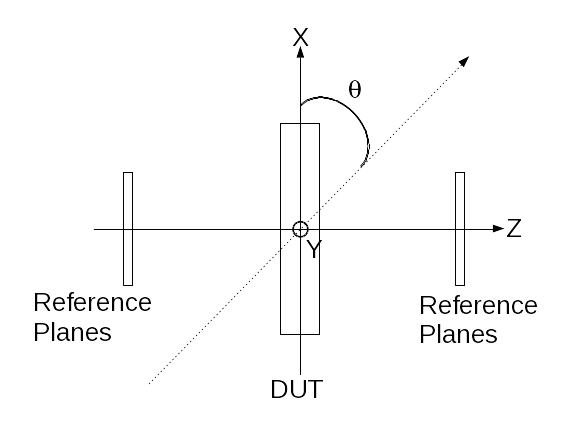
\includegraphics[width = 0.7\textwidth]{Pictures/deformation/lab_frame.png}
      \caption{Drawing of the laboratory coordinates.}
      \label{fig:labCoordinates}
    \end{figure}

    \subsection{Measurements}

    The prototype validation was done under several conditions.
    Firstly, three different geometric configurations were used.
    On the first one presented on the figure~\ref{fig:tbNormal}, the \gls{DUT} is parallel to the telescope planes and the beam is hitting the device in a normal incidence.
    The \gls{DUT} is placed in between the two arms.
    The middle of the foam is at equal distance from both inner telescope planes.
    For the second configuration, as shown on the figure~\ref{fig:tilt36}, the distance between the telescope planes are the same, but the \gls{DUT} is tilted between 28 and 40 degrees along the $y$-axis.
    Runs with a larger angle (60 degrees) were done.
    Due to the PLUME box's size, the cabling for the acquisition, the air cooling system and the design of the telescope stage, limiting the spacing between the two arms, the \gls{DUT} was placed behind the two arms, as presented on the figure~\ref{fig:tilt60}.
    For both configurations, different parameters were modified.
    The thresholds were set to 5 and 6 mV, different sensors were aimed and the air flow speed was set to 3 $\text{m.s}^{-1}$ and 6 $\text{m.s}^{-1}$.

    \begin{figure}[!h]
      \centering
      \begin{subfigure}[t]{0.9\textwidth}
        \centering
        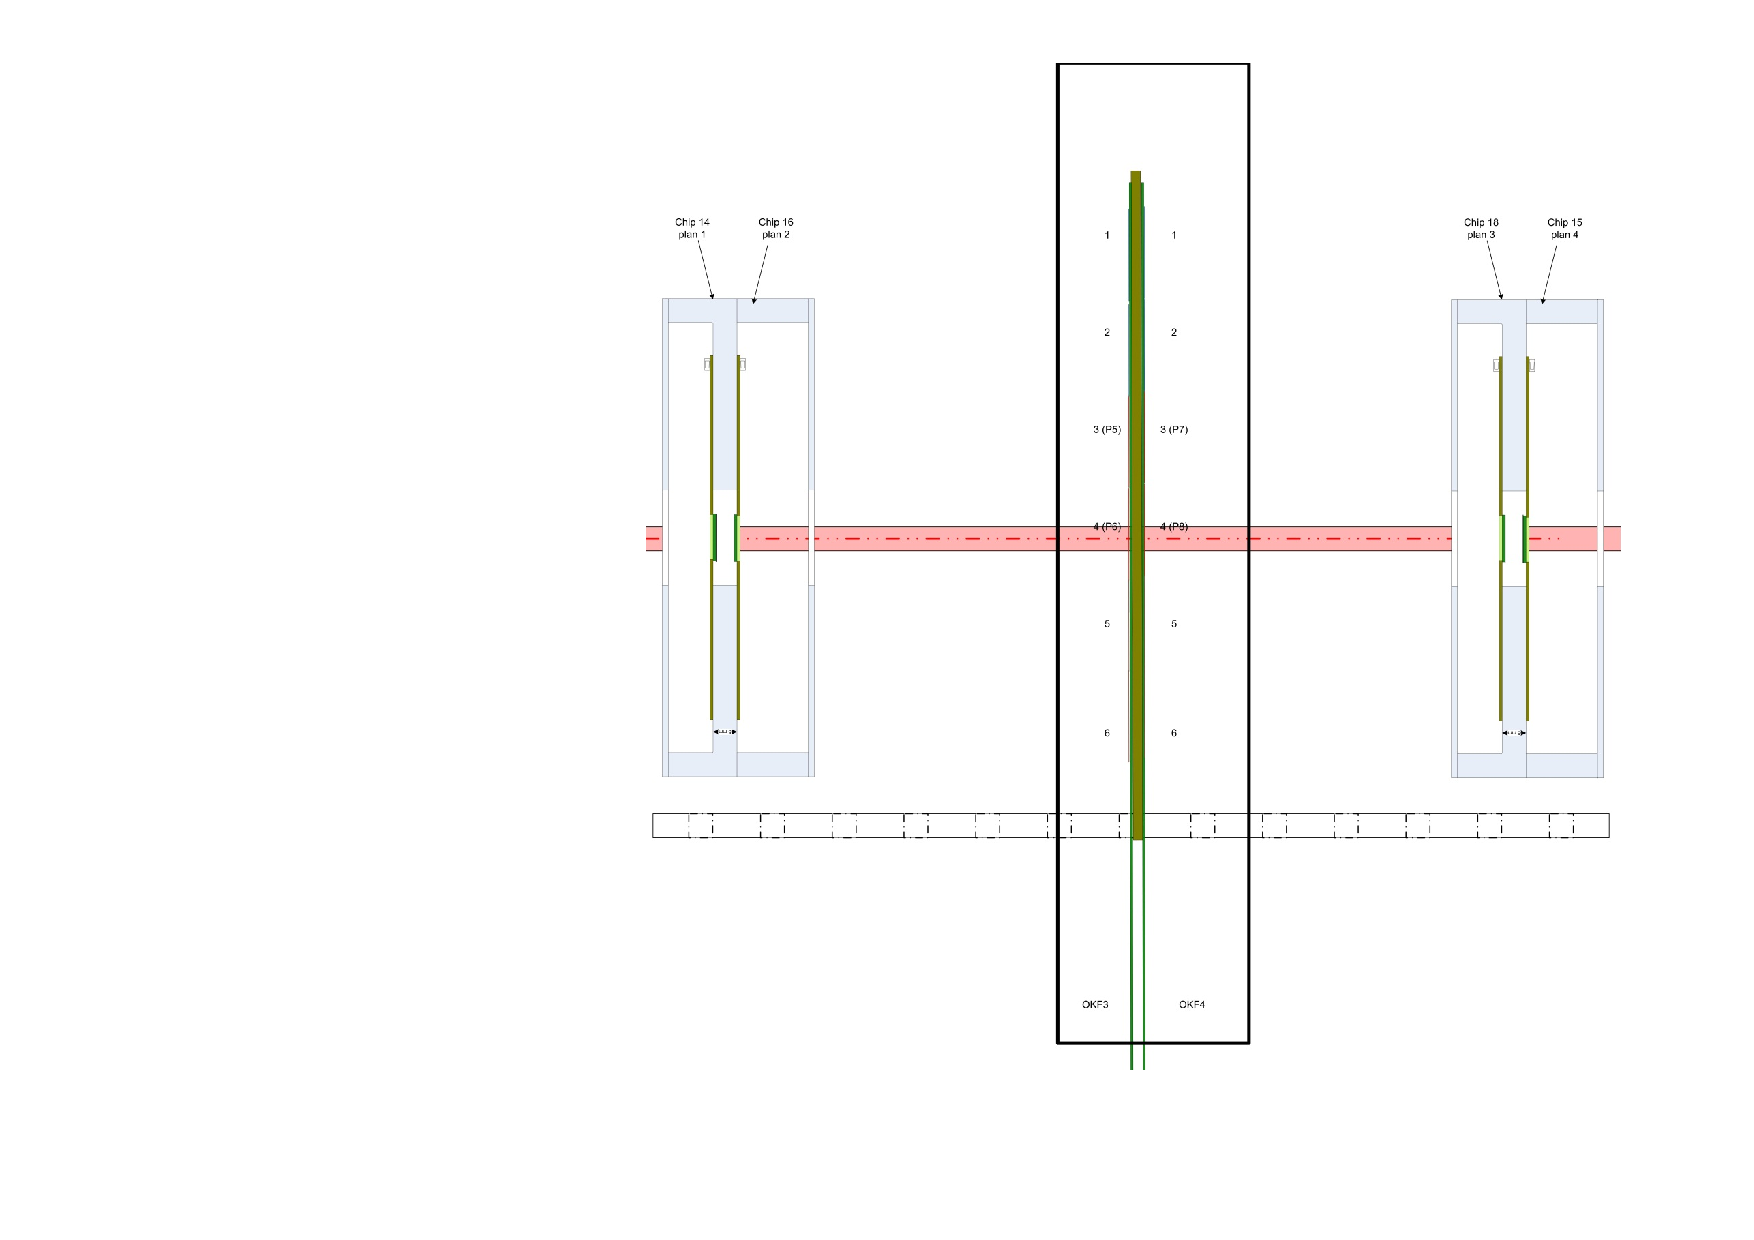
\includegraphics[width = 0.5 \textwidth]{Pictures/deformation/tb_cern_11_sketch_normal.pdf}
        \caption{Set-up for the PLUME ladder in normal incidence with respect to the beam direction.}
        \label{fig:tbNormal}
      \end{subfigure}

      \begin{subfigure}[t]{0.45\textwidth}
        \centering
        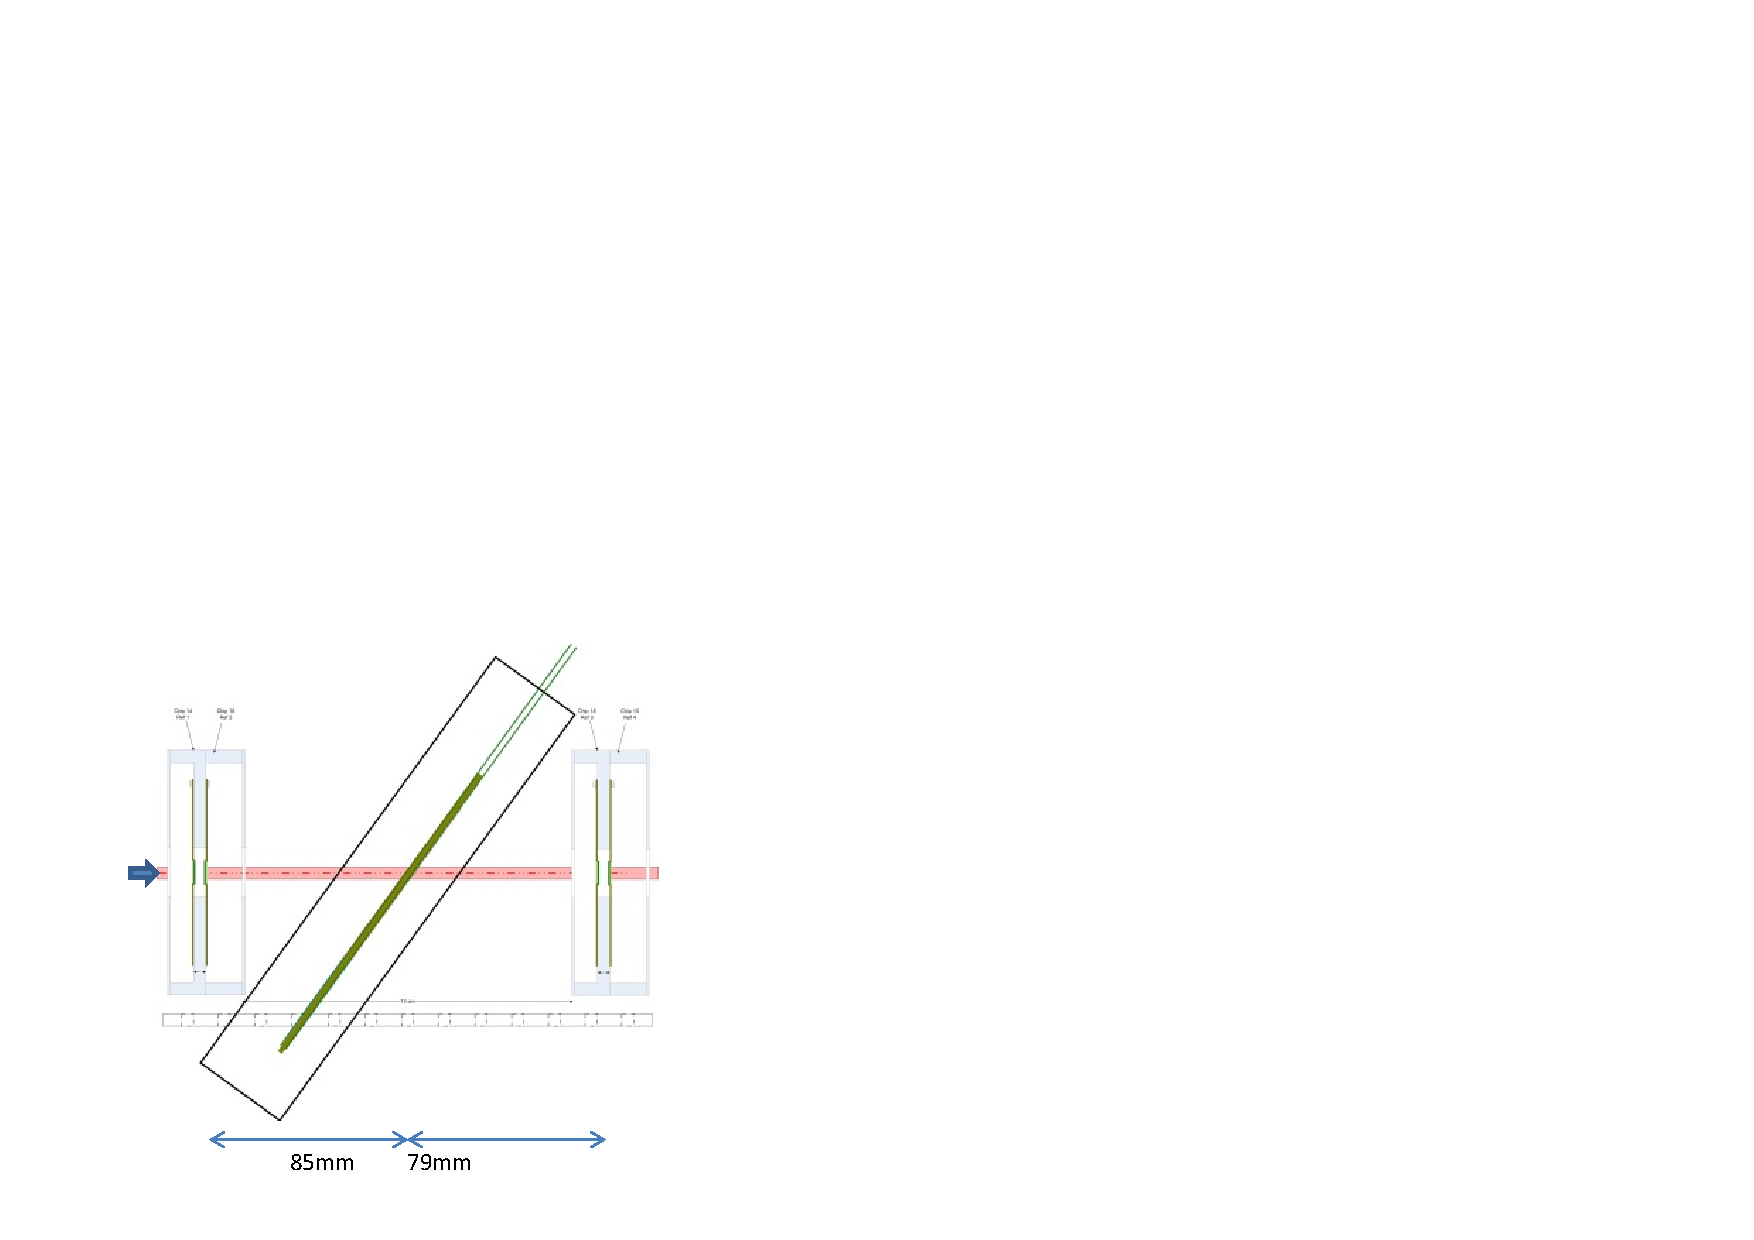
\includegraphics[width=0.8\textwidth]{Pictures/deformation/tb_cern_11_sketch_tilted.pdf}
        \caption{Configuration for an angle between 28 and 40 degrees.}
        \label{fig:tilt36}
      \end{subfigure}
      ~%\quad
       %add desired spacing between images, e. g. ~, \quad, \qquad, \hfill etc. 
        %(or a blank line to force the subfigure onto a new line)
      \begin{subfigure}[t]{0.45\textwidth}
        \centering
        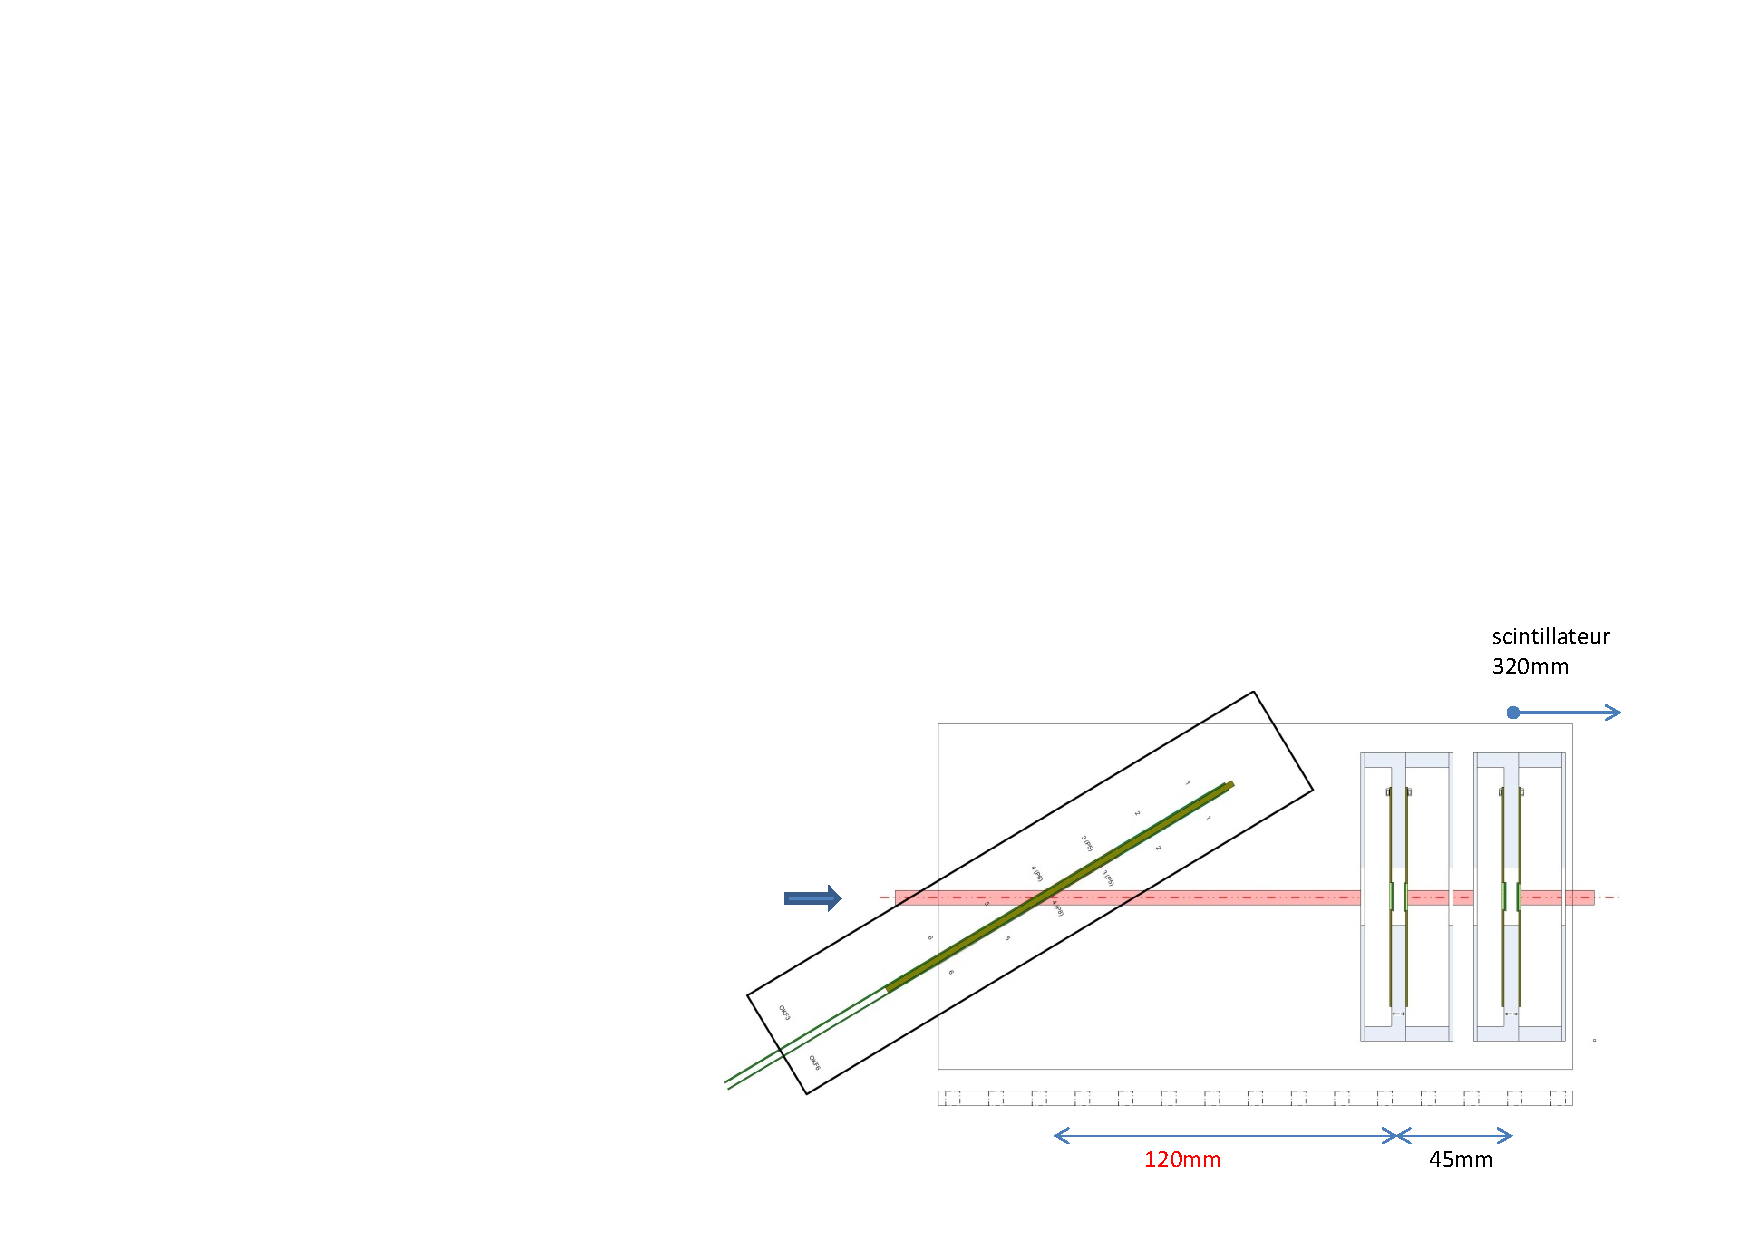
\includegraphics[width=0.95\textwidth]{Pictures/deformation/tb_cern_11_sketch_tilted120mm.pdf}
        \caption{Configuration for an angle of 60 degrees.}
        \label{fig:tilt60}
      \end{subfigure}
      \caption{Top view sketches of the test beam configuration for different ladder positions.}
      \label{fig:tilt}
    \end{figure}   

    The analysis and the results shown in the following sections were performed with \gls{TAF}, the analysis software developed by the IPHC and presented in chapter~\ref{chap:labTests}.

  \section{Spatial resolution studies}
   
    One of the measurements performed during the analysis is to determine the pointing resolution of the ladder.
    As the sensors used are well-known, the performance of the ladder should be similar to the one expected and the mechanical structure should not have an impact on the results.
    Any deviations on the pointing resolution or the efficiency might point out an unexpected effect of this mechanical structure on the whole system.
    %The sensors used are well-known and they should have a pointing resolution similar to the one expected, regardless the mechanical structure.
    %Any deviations might point out an impact of the mechanical structure on the whole system.
    The alignment steps to obtained the pointing resolution of the ladders are explained below for different run configurations. 

    \subsection{Normal incidence track}

    The sensors are sending to the acquisition the position of the pixel hit, on which frame this event was recorded, as well as the sensor ID.
    The binary file created contains no information about the relative position of each sensors.
    To perform an analysis, the telescope planes have to be aligned each other.
    The hit information of every plane are combined in order to create tracks. 
    A track correspond to the path of a particle through the system.
    Thanks to this information, the tracks are then compared to the hit position on the \gls{DUT} to give some information, such as the detection efficiency (the ratio of tracks matched to the hits on the \gls{DUT}), the spatial resolution (minimum distance to distinguish two incoming tracks).

    The alignment procedure is done in two steps: firstly the telescope planes are aligned to minimise the mismatch of particles' tracks and to improve the tracking resolution.
    Afterwards, the \gls{DUT} is aligned with respect to the information provided by the reference planes and then, the analysis itself is performed.
    Although the position of each sensors is measured during the test beam with a precision of the millimeter, for the analysis, a precision of the micron level has to be achieved.
    Three degrees of freedom were taken into account for the alignment here: two translations for the $x$ and $y$-axes and one rotation around the $z$-axis.
    The $z$ position is determined by the position measured during the test beam campaign and is not considered as a free parameter due to the beam used.

      \subsubsection{Alignment procedure and telescope alignment}

      Firstly, the data acquired during the test beam are processed to extract the signal and the hit information.
      For each frame, the position of the pixel(s) having a signal above the discriminator threshold is stored and assigned to an ID corresponding to a sensor.
      The analysis software is in charge to assign correctly the hit to the sensors and then to group the pixel fired into clusters.
      As the sensors used during the test beam have a binary output, no information on the seed pixel is available.
      Thus, the hit position is obtained from a centre of gravity calculation.

      Secondly, on the analysis software, one plane is considered as the origin of the telescope coordinate system and is used as a reference for the alignment.
      Usually, the first sensor hit by the beam is the main reference.
      The alignment means to correct the offset for the view angles and the hit position of the telescope planes and the \gls{DUT}.
      These offsets are found thanks to scatter plots where the residuals is represented as a function of predicted hit position.
      An alignment is considered as a good one when the residuals is not correlated to the predicted hit position.
      If it is not centered in zero, an offset has to be applied in this direction, whereas a slope indicates that a tilt has to be applied.
      First off, the hit position of the first plane are extrapolated to the next planes in order to perform the alignment.
      These tracks extrapolated are straight lines perpendicular to the hits position.
      Thus, the hit position of the last telescope plane are adjusted to match the hit position of the first plane.
      The alignment is an iterative procedure which consists to minimise the residual. 
      It corresponds to the distance between the extrapolated track to the closest hit on the sensor.
      Afterwards, the track candidates are built by matching a hit on the first plane to a hit on the last one.
      The second and third telescope planes are aligned with respect to the information provided by the extrapolated tracks.
      For example, the figure~\ref{fig:alignmentPlane2} and~\ref{fig:alignmentPlane3} show the residual distributions of the second and third planes in the $u$ and $v$ direction with respect to the tracks built by the first and the last planes.

      \begin{figure}
        \centering
        \begin{subfigure}[t]{0.45\textwidth}
          \centering
          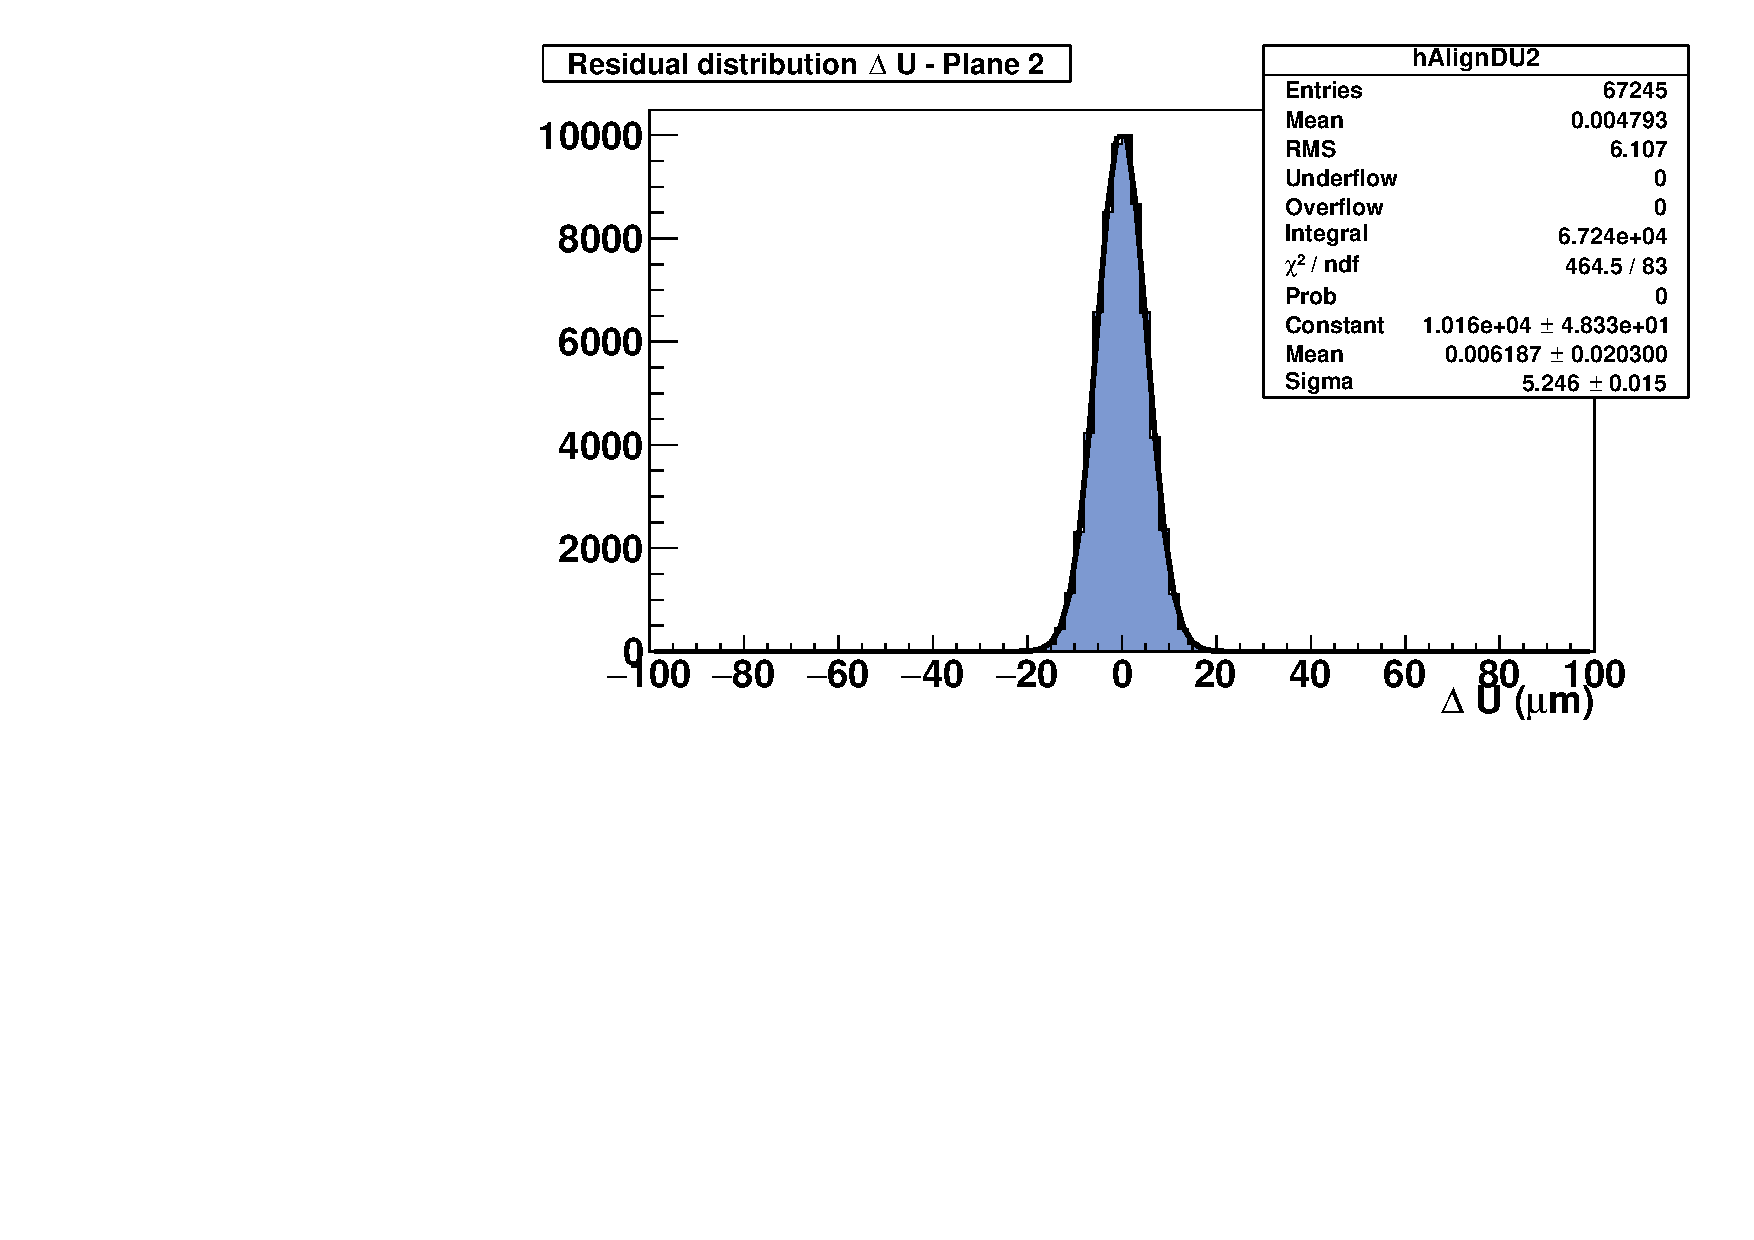
\includegraphics[width = 1.2\textwidth]{Pictures/deformation/residualUPl2_226056.pdf}
          \caption{Along $u$ direction.}
          \label{fig:alignmentPlane2}
        \end{subfigure}
        \hfill
         %add desired spacing between images, e. g. ~, \quad, \qquad, \hfill etc. 
          %(or a blank line to force the subfigure onto a new line)
        \begin{subfigure}[t]{0.45\textwidth}
          \centering
          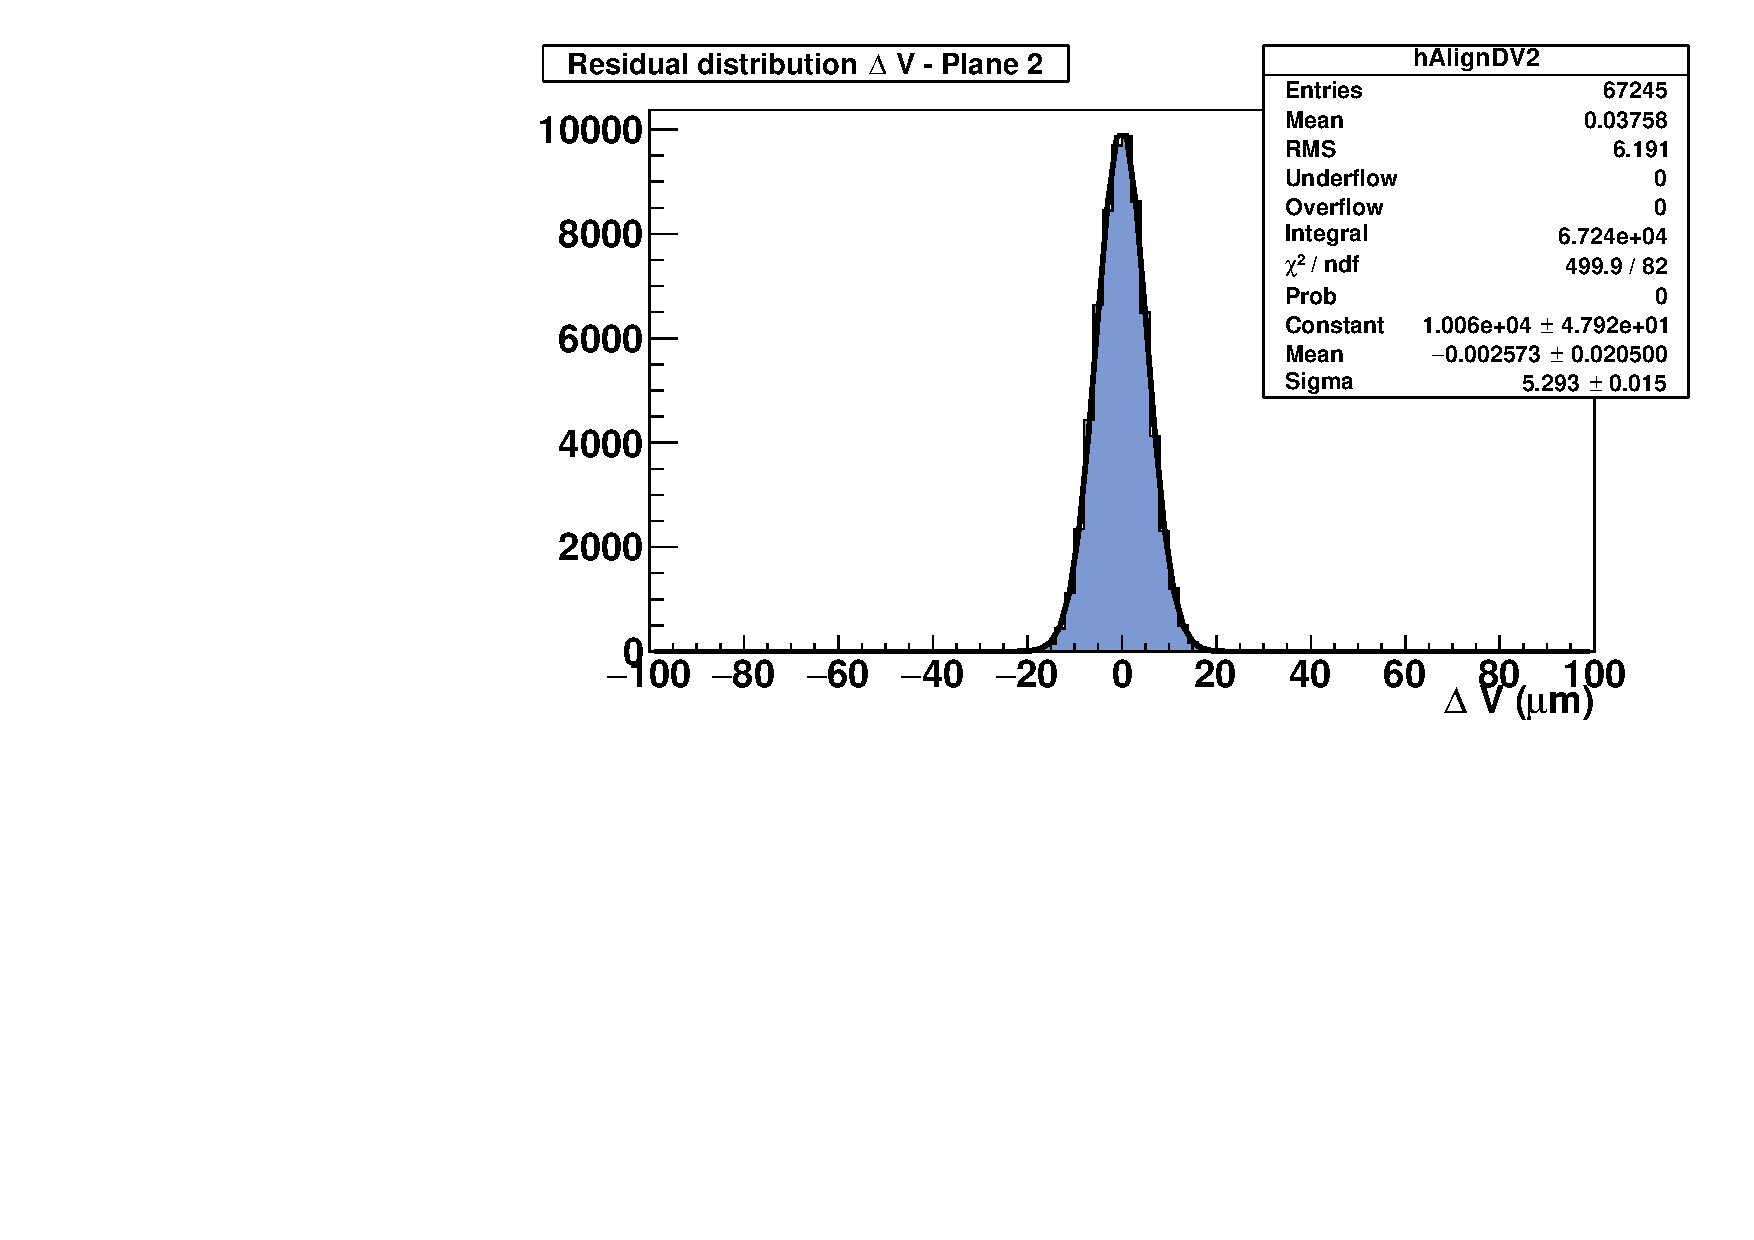
\includegraphics[width = 1.2\textwidth]{Pictures/deformation/residualVPl2_226056.pdf}
          \caption{Along $v$ direction.}
          \label{fig:alignmentPlane3}
        \end{subfigure}
        \caption{Residual distributions in the $u$ and $v$ directions for the middle telescope planes.}
        \label{fig:alignmentTelescope}
      \end{figure}

      As already explained, the alignment is an iterative procedure.
      To find a hit matching a track, a region of interest is defined.
      At the beginning, a hit in a $1000 \times 1000 \text{ }\mu\text{m}$ around the extrapolated one is search.
      Step by step, the region of interest is restricted to achieve a region of six times the pitch.
      
      After the telescope alignment is done, a track candidate is dismissed if it is made of less than four hits or if the $\chi^2$ fit is greater than a fixed value determined by the user. 
      For the alignment, two assumptions are defined. 
      The telescope planes are parallel each other.
      Thus the alignment consists of a translation along $x$ and $y$ and a rotation around the $z$-axis.
      As the test beam was performed without a magnetic field and pions of 120 GeV were used, the Coulomb multiple scattering is neglected.
      So, the tracks are perpendicular to the detectors and the alignment is not sensitive to the $z$ position.
      A precision of the millimeter level for the position does not have a huge impact on the alignment.

      \subsubsection{Alignment of the DUT}

      When the telescope alignment is done, the reference tracks reconstructed by the reference planes are used to align the \gls{DUT}.
      Its $z$ position is fixed, nonetheless, two degrees for freedom are added: the rotations along the $x$ and $y$-axes, plus the three other degrees of freedom defined above.
      To assist the user in the alignment steps, several plots are produced. 
      The figure~\ref{fig:UdeltaU} represents the residual in the $u$ direction as a function of the hit position on the plane in the same direction.
      The residual should not be correlated to the hit position on the plane.
      A slope or an offset indicates respectively a tilt in one direction and a shift in one direction.

      \begin{figure}
        %\centering
        \missingfigure{Delta-U = f(U)}
        \caption{Scatter plot of the residual in the $u$ direction as a function of the hit position on the plane in the same direction.}
        \label{fig:UdeltaU}
      \end{figure}

      \begin{figure}
        %\centering
        \missingfigure{Track-hit residual as a function of the hit position (normal incidence)}
        \caption{Distribution of the residuals for the DUT.}
        \label{fig:alignmentDUT}
      \end{figure}

      The figure~\ref{fig:alignmentDUT} shows the residuals distribution in both direction for one sensor of the \gls{DUT}.

      The resolution measured $\sigma_{Res}$ here is a combination of the resolution of the telescope $\sigma_{tel}$, the multiple scattering $\sigma_{M.S}$ and the pointing resolution of the sensor $\sigma_{DUT}$, as described in equation~\ref{eq:pointingResolution}.
      
      \begin{equation}
        \sigma_{Res}^2 = \sigma_{tel}^2 + \sigma_{DUT}^2 + \sigma_{M.S}^2
        \label{eq:pointingResolution}
      \end{equation}

      As the Coloumb multiple scattering is not relevant here due to the beam used, the pointing resolution of a \gls{DUT} sensor is then:

      \begin{equation}
        \sigma_{DUT} = \sqrt{\sigma_{tel}^2 - \sigma_{Res}^2}
      \end{equation}

      For the sensors studied here, the spatial resolution achieved is ... $\mu\text{m}$.

    \subsection{Ladder tilted in one direction}
    \label{subsec:deformation}

      The same alignment procedure as presented above, was applied for runs where the ladder was tilted with respect to the beam direction, as shown on the figure~\ref{fig:tilt}.
      For the run studied here, the tilt is ...degrees, the threshold ... and the air flow speed ...$\text{m.s}^{-1}$.
      As the telescope was not moved between the normal incidence run and this one, the alignment performed before is kept.
      Nevertheless, the \gls{DUT} alignment procedure is more complicated. 
      First of all, the scatter plot, shown on figure~\ref{fig:scatterDUU}, representing the residual in the $u$-direction as a function of the hit position on the plane in the same direction, has a different shape.
      This plot shows a banana shape, that can not been reduced by simple offset and tilts.
      The residual distribution obtained after trying to align the \gls{DUT} gives a residual wider with large tails, as seen on the figure~\ref{fig:residualDef}

      \begin{figure}
        %\centering
        \missingfigure{Scatter plot deformed}
        \caption{Scatter plot of the residual in the $u$-direction as a function of the hit position in the same direction.}
        \label{fig:scatterDUU}
      \end{figure}

      \begin{figure}
        %\centering
        \missingfigure{Track-hit residual }
        \caption{Distribution of the track-hit residual.}
        \label{fig:residualDef}
      \end{figure}

      As the tilt is applied in only one direction, the scatter plot in the $v$-direction, as well as the residual distribution are not affected by this behavior. 
      The results obtained are of the same order as the one expected for the normal incidence ladder.
    
      \subsubsection{Origin of the deviations}

      The deviations observed here are mainly caused by the characteristics of the ladder.
      Indeed, ultra-thin sensors with a thickness of approximately $50 \text{ }\mu\text{m}$ are used.
      Naturally, without any mechanical structure, the sensors tend to be very flexible.
      Nevertheless, the gluing procedure to the flex-cable and the \gls{SiC} foam induces permanent deformations of the surface of about $10 \text{ }\mu\text{m}$ that can not be flatten.
      Also, the foam has an open-cell structure with small bumps and the glue spots might be more or less important on some positions.
      The Bristol group has performed a mechanical survey on a mechanical prototype.
      This prototype has non-functioning MIMOSA-20 sensors that were thinned and attached to the standard flex-circuits.
      The measurements done with an optical survey equipment have revealed a peak-to-peak flatness of the order of the $100 \text{ }\mu\text{m}$ on both side.
      The figure~\ref{fig:mechanicalSurvey} shows the result of this survey.
      The overall shape is due to the intrinsic shape of the foam.
       
      \begin{figure}[!h]
        \centering
        \begin{subfigure}[t]{0.45\textwidth}
          \centering
          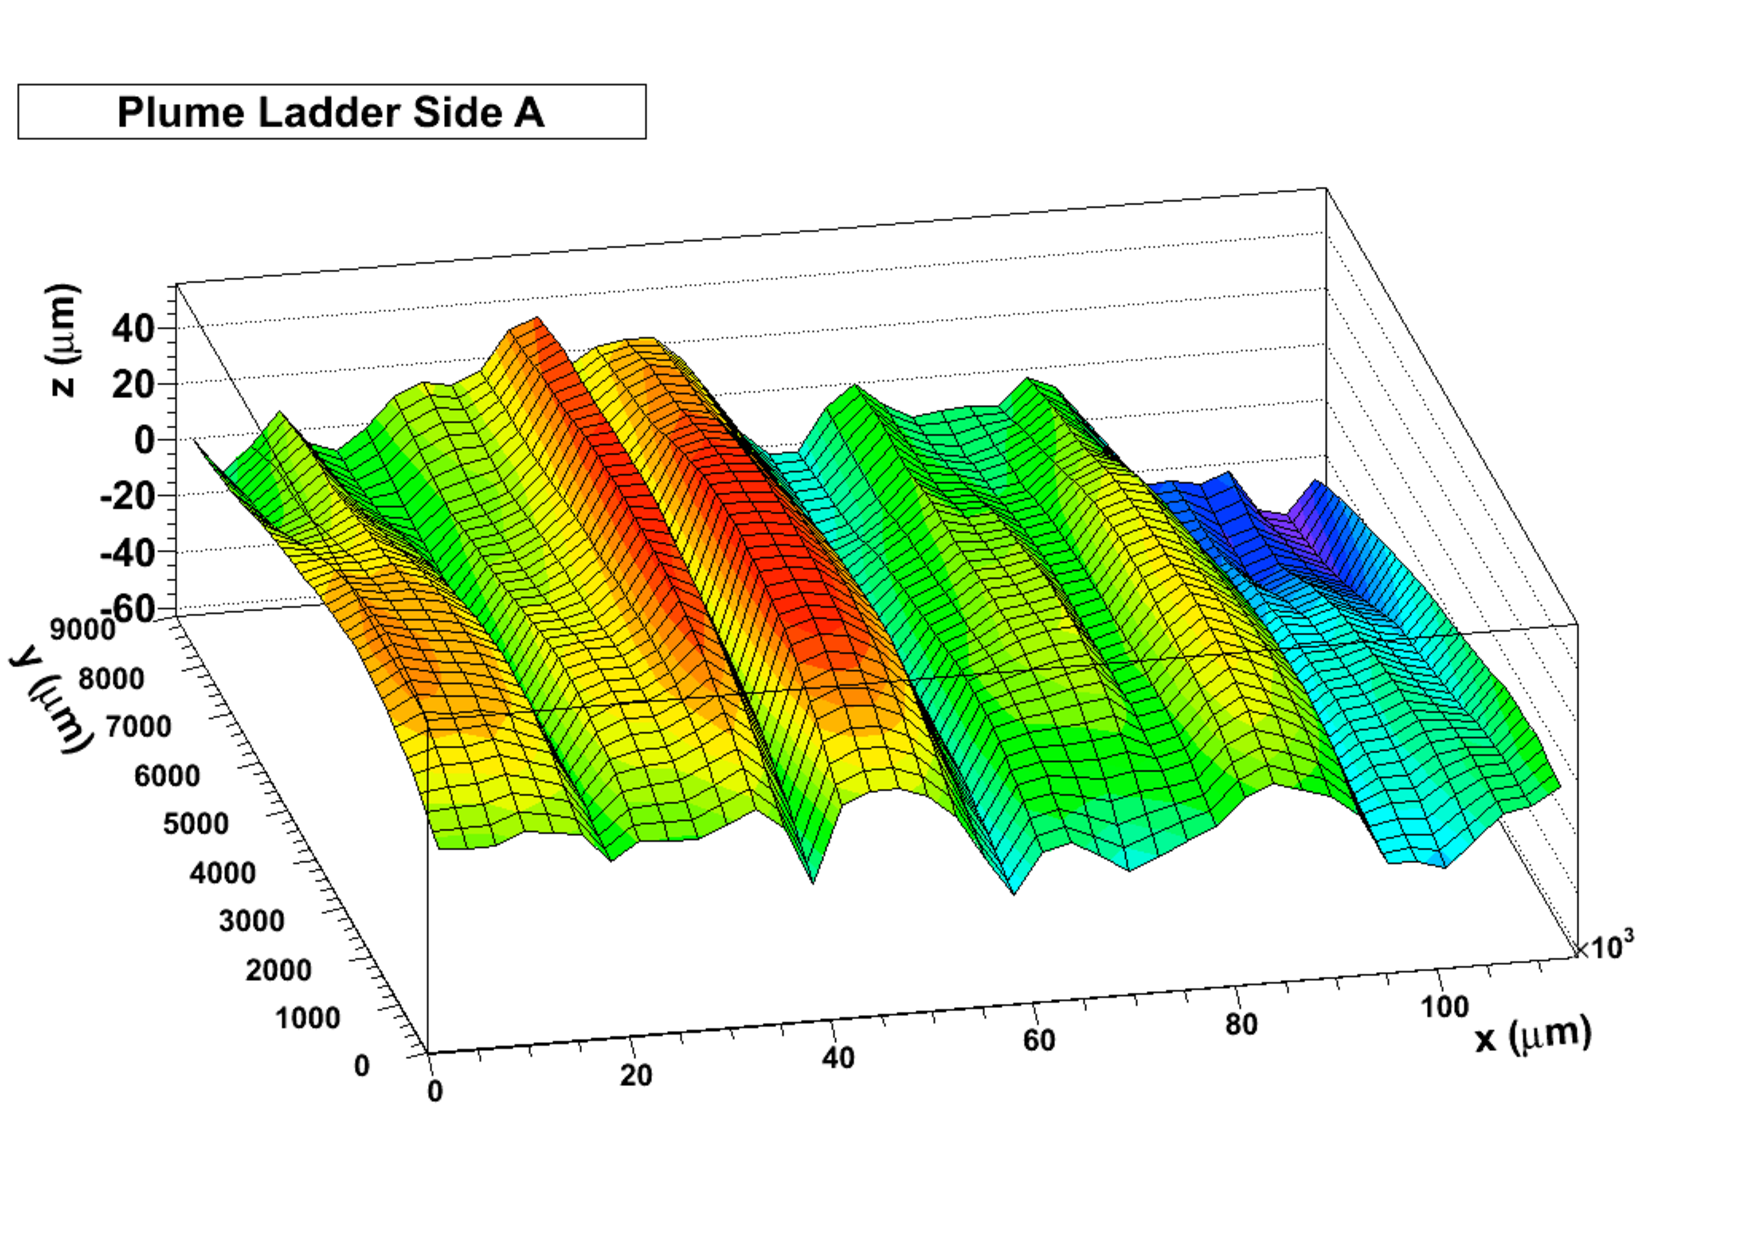
\includegraphics[width = 1.2\textwidth]{Pictures/deformation/surveyResults.pdf}
        \end{subfigure}
        \hfill
         %add desired spacing between images, e. g. ~, \quad, \qquad, \hfill etc. 
          %(or a blank line to force the subfigure onto a new line)
        \begin{subfigure}[t]{0.45\textwidth}
          \centering
          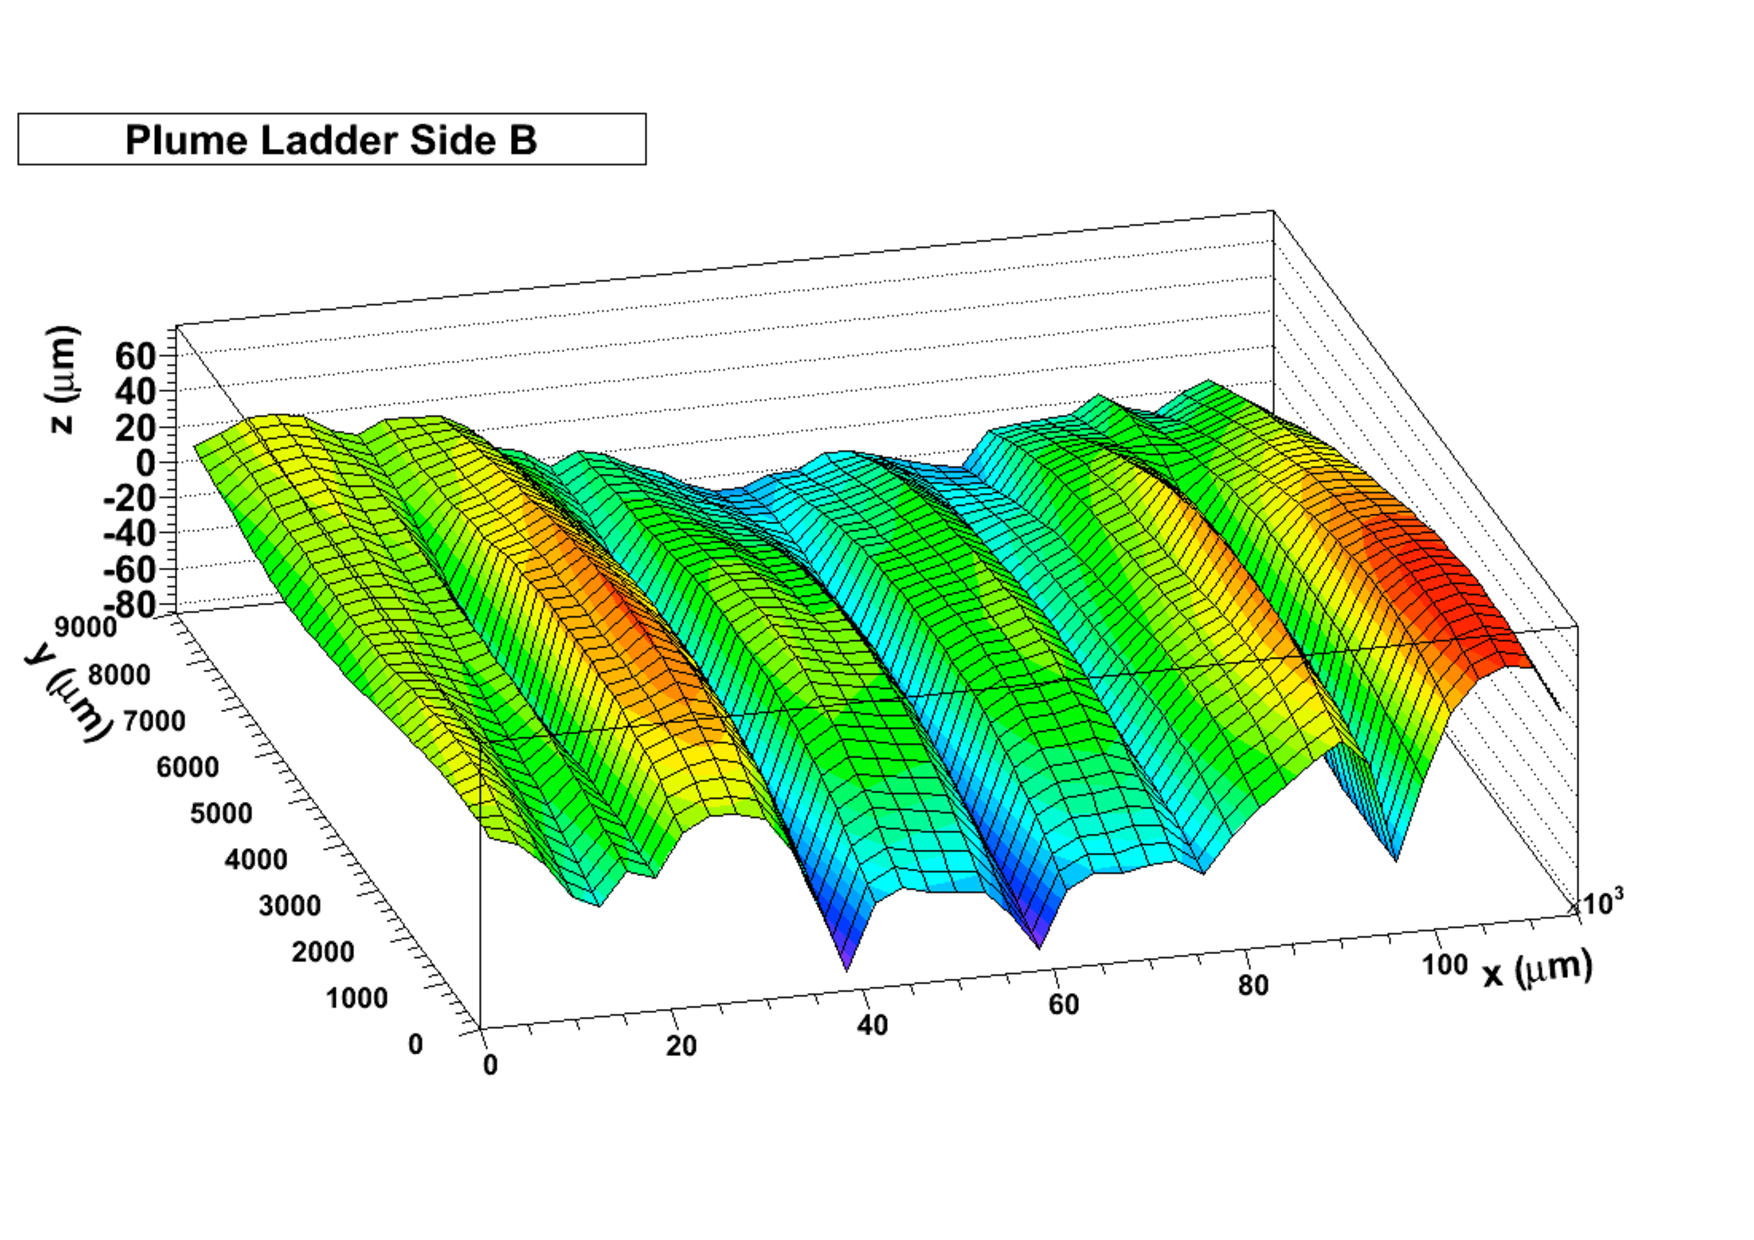
\includegraphics[width = 1.2\textwidth]{Pictures/deformation/surveyResultsB.pdf}
        \end{subfigure}

        \caption{Results of the mechanical survey of each side of the PLUME mechanical prototype.}
        \label{fig:mechanicalSurvey}
      \end{figure}

      During the analysis, this non-flatness structure is not taken into account.
      The sensors are modelled as completely flat planes and the $z$ position is fixed.
      However, the sensor position in three dimensions is actually different due to the deformations.
      When the particles are not striking the sensor in normal incidence, the hit predicted with respect to the flat plane does not have the same position anymore.
      Thus, the residual between the position of the extrapolated track and the predicted hit is increasing.
      The figure~\ref{fig:originDef} depicts the difference between the hit expected $U_{h}$ on the flat plane and the extrapolation of the actual hit $U'_{\text{h extrapolated}}$.
      For a normal incidence, this two hits are at the same position, but larger is the angle, larger is the difference between the expected hit and the extrapolated one.
      The deformation height $\delta w$ can be expressed as a function of the angle $\theta$ and the residual $\delta u$ of the track:

      \begin{equation}
        \delta w = \frac{\delta u}{\tan(\theta)}
      \end{equation}

      Thus, the deformation of the surface is sensitive to the angle of the incoming track.

      \begin{figure}[!h]
      \centering
        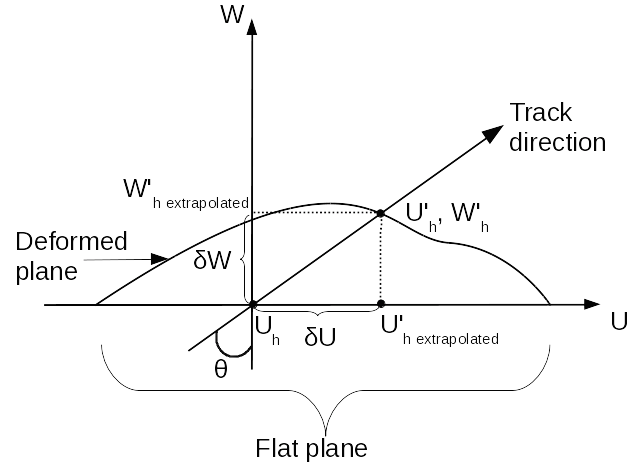
\includegraphics[width = 0.8\textwidth]{Pictures/deformation/origin_deformation.png}
        \caption{Side view of the sensor's deformation....}
        \label{fig:originDef}
      \end{figure}

      \subsubsection{Algorithm to estimate the deformations}

      The sensor deformation was already studied in Strasbourg by Maria Robert Daniel.
      The sensor was mapped for the alignment in order to remove the contribution of the deviation on the residual\cite{maria}.
      As this method is done manually and is time consuming, an automatic method has to be implemented.

      A similar effect was observed in the CMS tracker during the alignment procedure with cosmic rays and a method was developed to compensate the deformations\cite{CMSalignment}. 
      By using modified two-dimensions Legendre polynomials to parametrise the sensors' deformations, they were able to minimise the effect of the deviations.
      During the PLUME test beam, the tilt was only in one direction, thus, the deformation in the other direction is not accessible.
      A similar method was implemented in TAF.

      As tracks with a large angle of incidence are more sensitive to the exact position of the plane in three dimensions, the coordinates of the hits have to be exactly known.
      The deviations of the track-hit residual distribution provided an information on the behaviour of the deformation.
      Thus, the hit position is determined during the analysis with the extrapolation of the sensor's surface shape.
      To determine more precisely the hit position during the analysis, the deviations need to be used. 
      The distribution of the track-hit residuals as the function of the hit position is profiled and then fitted with a Legendre function. 
      Each coefficient given by the fit procedure are used to calculate the new hit position thanks to Legendre polynomials

      \begin{figure}
        %\centering
        \missingfigure{Profile of track-hit residual as a function of the hit position}
        \caption{Profile of the scatter plot showing the track-hit residual in the $u$-direction as a function of the hit position on the plane for the same direction. The profile is then fitted with Legendre polynomials.}
        \label{fig:profileFitted}
      \end{figure}

      \begin{equation}
        w\left(u_{r}\right) = \sum_{k=0}^n \omega_{k}P_{k}\left(u_{r}\right)
        \label{eq:polynomials}
      \end{equation}

      Where $u_{r}$ is the hit position on the sensor along the $u$-direction and normalised to the sensor width, $\omega_{k}$ are the coefficients that quantify the sensor curvature and $P_{k}(u_{r})$ are the Legendre polynomials defined by the equation~\ref{eq:Legendre}:

      \begin{equation}
        P_{k}\left(u_{r}\right) = \frac{1}{2^{k}!}\frac{d^{k}}{du_{r}^{k}} \left( (u_{r}^2 - 1)^{k}\right)
        \label{eq:Legendre}
      \end{equation}

      \begin{figure}
        %\centering
        \missingfigure{Residual after correction}
      \end{figure}

      \subsubsection{Correction of the deformation}

      The scatter plot displayed in subsection~\ref{subsec:deformation} was profiled and fitted with a Legendre function.
      The figure~\ref{fig:scatterFitted} depicts the fit results. 
      The coefficients of this fit are used to calculate again the position of each hit.
      The alignment is run again and the deviation effects are minimised on the scatter plot (see figure~\ref{fig:scatterCorrected}).
      Nevertheless, the plot edges still show small deviation.\todo{Why?}
      Regarding the residual distribution, the spatial residual obtained is now ... instead of ... .

      \begin{figure}
        %\centering
        \missingfigure{Scatter plot fitted}
        \caption{Scatter plot fitted}
        \label{fig:scatterFitted}
      \end{figure}

      \begin{figure}
        %\centering
        \missingfigure{Scatter plot after correction}
        \caption{Scatter plot obtained after applying the correction.}
        \label{fig:scatterCorrected}
      \end{figure}

      This method was applied for different angles and the results is summarised in the table~\ref{tab:correctionOfDeformation}. 
      The correction based on Legendre polynomials shows good results for the 28 degrees angle with a pointing resolution of ... .
      Although for larger angles the precision is not expecting to reach the normal value, the results obtained are less positive.
      For the large angle (60 degrees), the position of the \gls{DUT} on the outside of the telescope arms does not provide a good telescope resolution.
      It was measured to be .... .
      It can be seen that more important is the angle, less the spatial resolution is good. 

      \begin{table}
        \begin{tabular}{|c|c|c|c|c|}
          \hline %----------------------------------------------------------------------------------------------------------------
          %Run Number  &  Plane Number &  Fan speed (m/s)   & Tilted angle  &   $\sigma_{U}^{Def}$ ($\mu m$) &   $\sigma_{U}^{Cor}$ ($\mu m$) & $\sigma_{U}^{DUT}$ ($\mu m$)\\
          %Side &  Tilted angle  &   $\sigma_{U}^{Def}$ ($\mu m$) &   $\sigma_{U}^{Cor}$ ($\mu m$) & $\sigma_{U}^{DUT}$ ($\mu m$)\\
          Side &  Tilted angle  &   $\sigma_{U}^{Def}$ ($\mu m$) &   $\sigma_{U}^{Cor}$ ($\mu m$) & Improvement \\
          \hline %----------------------------------------------------------------------------------------------------------------
          \hline %----------------------------------------------------------------------------------------------------------------
          %Front   & 3         &      28       &      9.586 &      5.568                       &    5.115           \\
          %Back    & 3         &      28       &      6.507 &      5.533                       &    5.077           \\
          %\hline %----------------------------------------------------------------------------------------------------------------
          %Front &      28       & $ 8.8 \ \pm \ 0.08 $ & $ 4.8 \ \pm \ 0.05 $ &    4.3  \\
          %Back  &      28       & $ 5.6 \ \pm \ 0.07 $ & $ 4.5 \ \pm \ 0.05 $ &    3.9  \\
          Front &      28       & $ 8.8 \ \pm \ 0.1 $ & $ 4.8 \ \pm \ 0.1 $ &    $45.5 \ \%$  \\
          Back  &      28       & $ 5.6 \ \pm \ 0.1 $ & $ 4.5 \ \pm \ 0.1 $ &    $19.6 \ \%$ \\
          %\hline %----------------------------------------------------------------------------------------------------------------
          \hline %----------------------------------------------------------------------------------------------------------------
          %Front &      36       & $ 13.4 \ \pm \ 0.1 $ & $ 6.3 \ \pm \ 0.08 $ &    5.9               \\
          %Back  &      36       & $ 6.5 \ \pm \ 0.09 $ & $ 6.8 \ \pm \ 0.09 $ &    6.4           \\
          Front &      36       & $ 13.4 \ \pm \ 0.1 $ & $ 6.3 \ \pm \ 0.1 $ &    $52.9 \ \%$               \\
          Back  &      36       & $ 7.5 \ \pm \ 0.1 $ & $ 6.8 \ \pm \ 0.1 $ &    $9 \ \%$          \\
          %\hline %----------------------------------------------------------------------------------------------------------------
          \hline %----------------------------------------------------------------------------------------------------------------
          Front &      60       & $ 41.2 \ \pm \ 0.15$ & $25.8 \ \pm \ 0.2$  &    $37.4 \ \%$              \\
          Back  &      60       & $ 23.3 \ \pm \ 0.13$ & $21.7 \ \pm \ 0.1$  &    $6.8 \ \%$           \\
          \hline %----------------------------------------------------------------------------------------------------------------
        \end{tabular}
        \caption{Alignment results for different angles before and after using the correction based on Legendre polynomials.}
        \label{tab:correctionOfDeformation}
      \end{table}

      An hypothesis on the deformation of the origin might come from heating or the cooling system that induces vibration.
      Although few runs were performed with a different air flow speed, the impact of the cooling system and the heat was not planned for this test beam.
      Thus, the results are not relevant enough to conclude for any vibration, or the heat that tends to deform more the surface.
    
  \section{Benefits of double-sided measurement}
  
  As two modules are sharing the same mechanical structure, the information provided by each sides can be combined together.
  A mini-vector is created by connecting two hits on each side of the ladder for the same event.
  This combination gives access to a new information compared to a single sensor: the angular resolution.

    \subsection{Spatial resolution with mini-vectors}

    To study the benefits of the mini-vector, a virtual intermediate plane is defined at the center of the ladder.
    The two hits of each side of the \gls{DUT} are connected to form a mini-vector and the intersection of this vector to the intermediate plane is determined.
    The intersection of the extrapolated track to the intermediate plane is also performed and the distance between the position of the track and the position of the mini is then measured.

    \begin{figure}[!h]
      \centering
      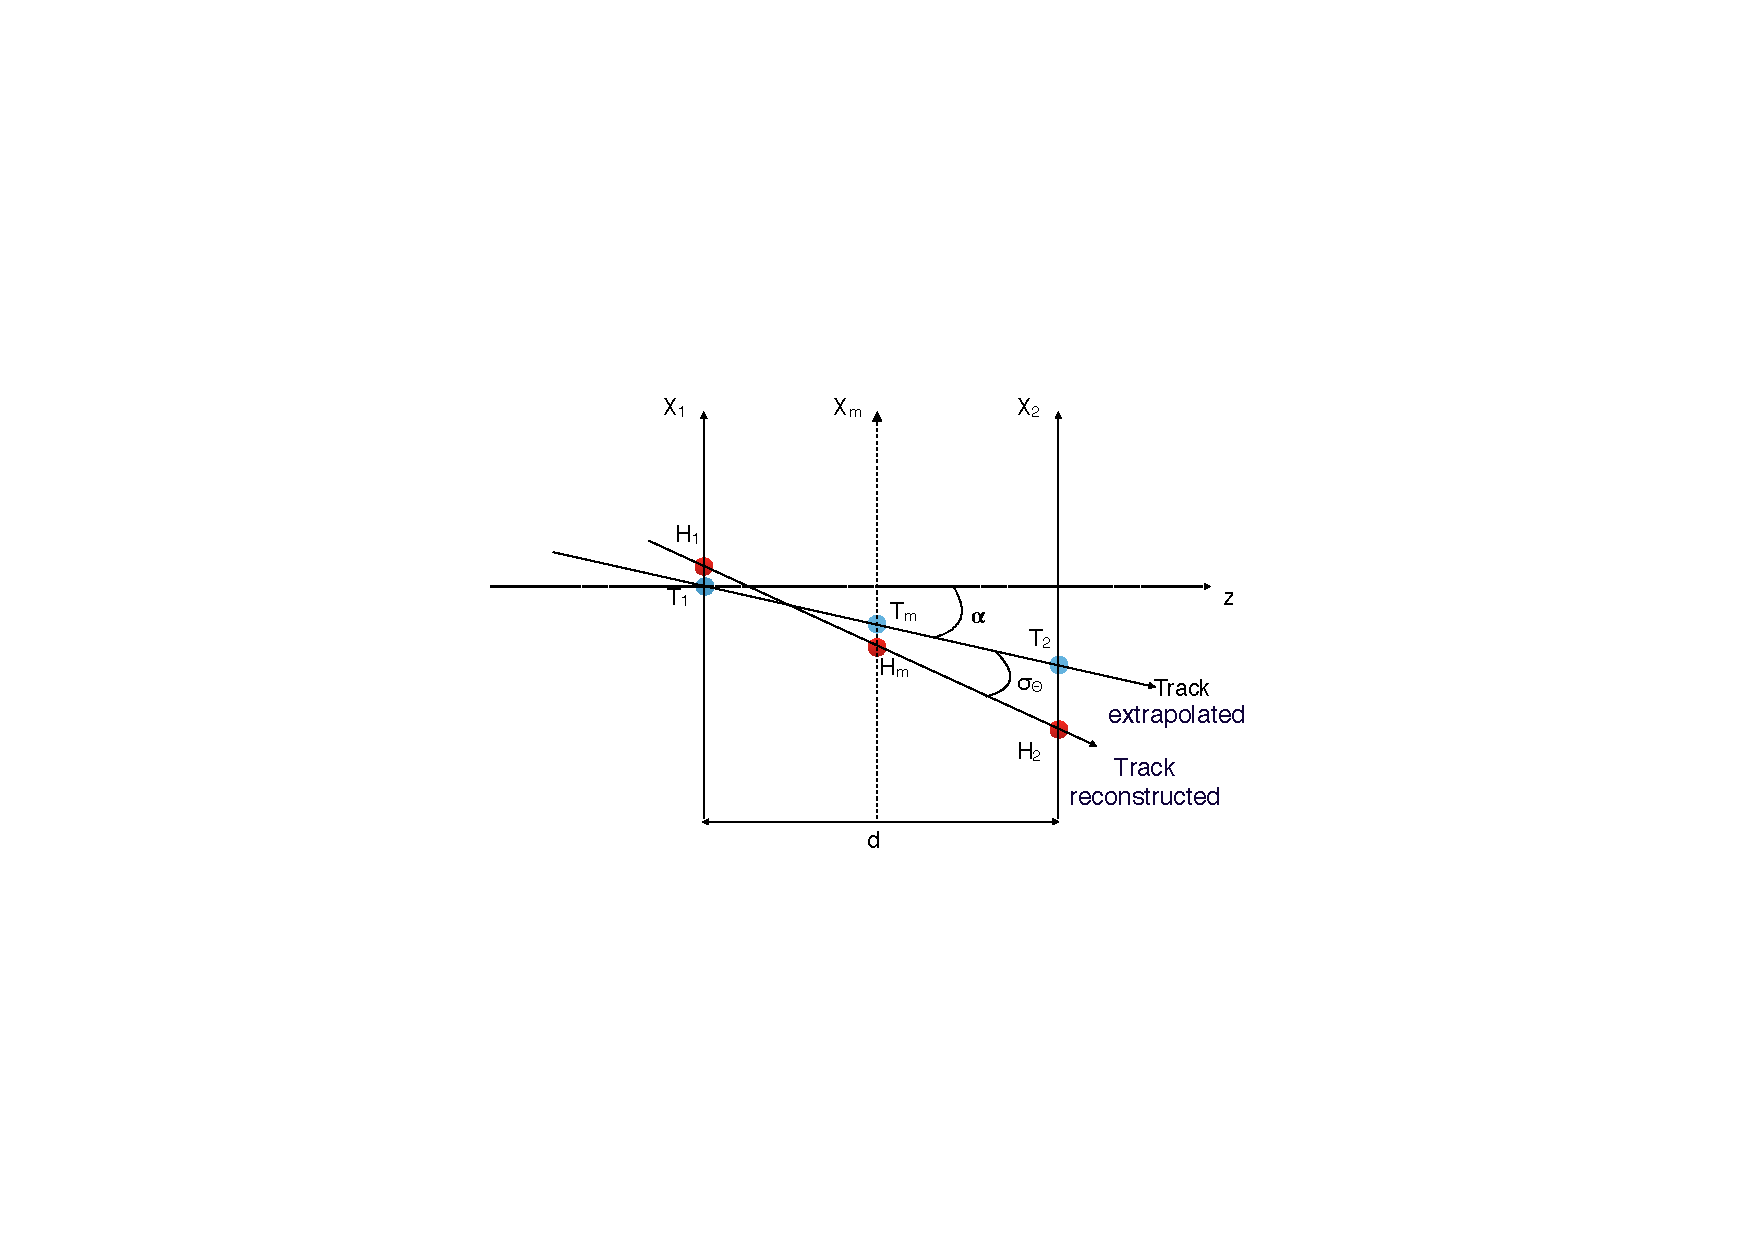
\includegraphics[width=0.7\textwidth]{Pictures/deformation/mini_vectors.pdf}
      \caption{Principle of the mini-vector. The two hits (in red) on the planes $x_1$ and $x_2$ are connected and the intersection on virtual intermediate plane $x_m$ is then determined. The blue points represents the track extrapolated through the DUT. }
      \label{fig:MV}
    \end{figure}

    A theoretical estimation of the spatial resolution for the mini-vector can be done thanks to the formula above:

    \begin{equation}
      \sigma_m^2 = \frac{\sigma_{front}^2 + \sigma_{back}^2}{(d_{front} - d{back})^2}*d_{m}^2 + \sigma_{tel}^2
      \label{eq:resolutionMV}
    \end{equation}

    Where $\sigma_m$ is the resolution on the intermediate plane, $\sigma_{front}$ and $\sigma_{back}$ are the resolution of the two sides of the \gls{DUT}, $\sigma_{tel}$ the resolution of the telescope and $(d_{front} - d_{back})$ the distance between the front and back planes and $d_{m}^2$ the position of the intermediate plane.
    For the plume ladder, the \gls{SiC} as a thickness of 2 mm and the intermediate plane is located in the middle, the equation~\ref{eq:resolutionMV} can be rewritten:

    \begin{equation}
      \sigma_m^2 = \frac{\sigma_{front}^2 + \sigma_{back}^2}{4} + \sigma_{tel}^2
    \end{equation}

    Thus, if the resolution on both side of the telescope are similar with $\sigma_{front} = \sigma_{back} = \sigma$, the resolution of the mini-vector $\sigma_{res}$ is then:

    \begin{equation}
      \sigma_{res} = \frac{\sigma}{\sqrt{2}}
    \end{equation}

    \begin{figure}[!h]
      \centering
      \begin{subfigure}[t]{0.45\textwidth}
        \centering
        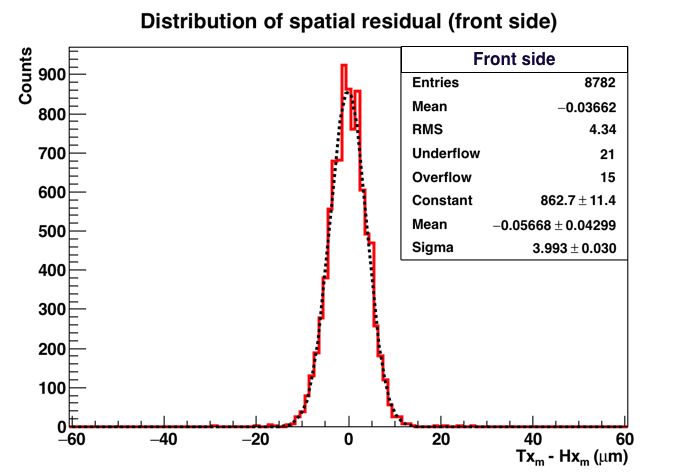
\includegraphics[width = 1.2\textwidth]{Pictures/deformation/hxtxFront_226056.png}
      \end{subfigure}
      \quad
       %add desired spacing between images, e. g. ~, \quad, \qquad, \hfill etc. 
        %(or a blank line to force the subfigure onto a new line)
      \begin{subfigure}[t]{0.45\textwidth}
        \centering
        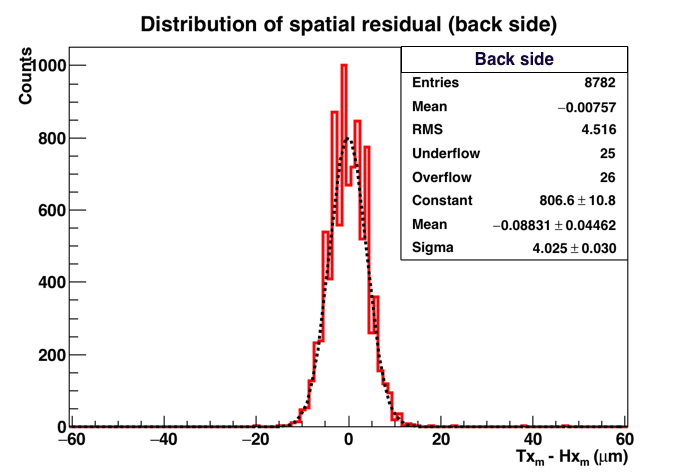
\includegraphics[width = 1.2\textwidth]{Pictures/deformation/hxtxBack_226056.png}
      \end{subfigure}
      \caption{Residual distribution for both side of the ladder in the $u$-direction}
      \label{fig:residualFrontBackLadder}
    \end{figure}

    For a run in normal incidence, the spatial resolution measured on each side is $\sigma_{front} \simeq \sigma_{back} \simeq 4 \text{ }\mu\text{m}$, according to the figure~\ref{fig:residualFrontBackLadder}.
    The resolution of the mini-vector should be then $\sigma_{res} \simeq 2.8 \text{ }\mu\text{m}$.
    The measurement of the residual for the mini-vector displayed on the figure~\ref{fig:residualMV} gives a residual of 3.2 $\mu\text{m}$.
    Taking into account the resolution of the telescope, the spatial resolution achieved by the mini-vector is $\sigma_res{} \simeq 2.9 \text{ }\mu\text{m}$.

    \begin{figure}[h]
      \centering
      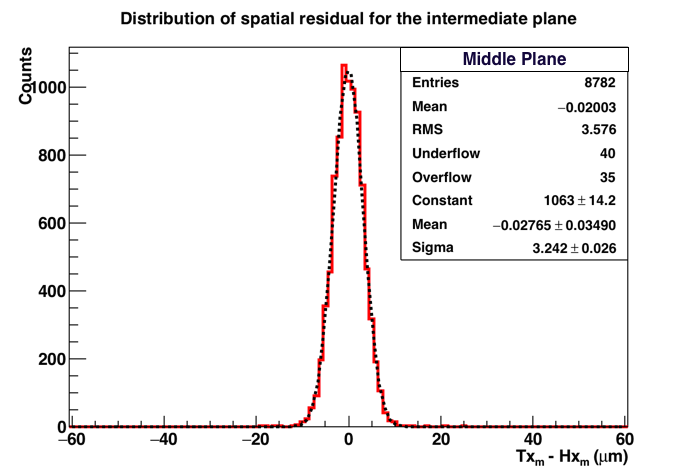
\includegraphics[width = 0.7\textwidth]{Pictures/deformation/hDiffPosX_226056.png}
      \caption{Residual distribution of the mini-vector measured on the intermediate plane.}
      \label{fig:residualMV}
    \end{figure}

   \subsection{Angular resolution}

   The mini-vectors give an access to new information not provided by a single sensor, the angular resolution.
   The direction of the track can be compared to the direction of the mini-vector.
   The estimation of the angular resolution is given by:

   \begin{equation}
     \sigma_{theta} = \frac{\sqrt{\sigma_{front}^2 + \sigma_{back}^2}}{d}
     \label{eq:angularResolution}
   \end{equation}

   With $\sigma_{front}$ and $\sigma_{back}$ the spatial resolution on each side of the \gls{DUT} in microns and d the distance between the two sides in microns.
   The spatial resolution here is $\sigma \simeq 3.6 \text{ }\mu\text{m}$ and the distance between the two planes 2000 microns.
   The angular resolution estimated is then $\sigma_{\theta} = 0.146^{\degree}$.  
   
   \begin{figure}[!h]
     \centering
     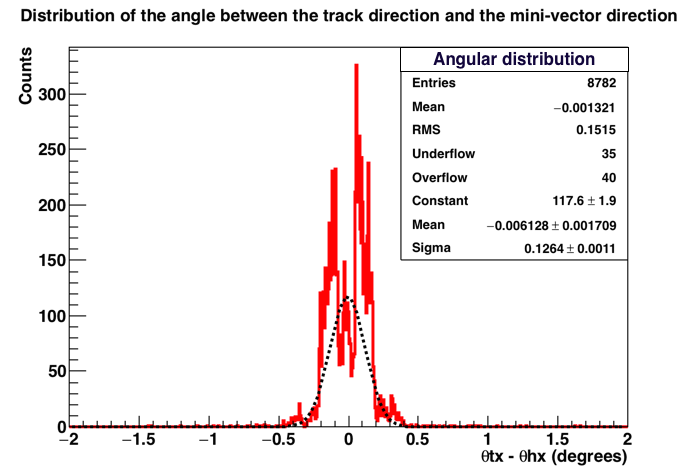
\includegraphics[width = 0.7\textwidth]{Pictures/deformation/hDiffAngleX_226056.png}
     \caption{Distribution of the angle between the tracks direction and the mini-vectors direction.}
     \label{fig:angRes}
   \end{figure}

   The figure~\ref{fig:angRes} depicts the distribution of the angle between the tracks direction and the mini-vectors direction.
   As it can be seen, several peaks are present and the distribution can't be extrapolated by a Gaussian fit.
   The sensors have a binary output and the hit position is determined by the centre-of-gravity of the clusters.
   If the cluster is only one pixel, the centre-of-gravity will be in the middle of the pixel, but if the clusters contain more pixels, this centre-of-gravity will be displaced.
   Moreover, the are some deviations in the distance between the hit projected to one side to the real hit position on this side.
   The figure~\ref{fig:clusterSize} represents the minimum distance between one cluster on one side to the cluster on the other side.
   
   \begin{figure}[!h]
     \centering
      \begin{subfigure}[t]{0.45\textwidth}
         \centering
         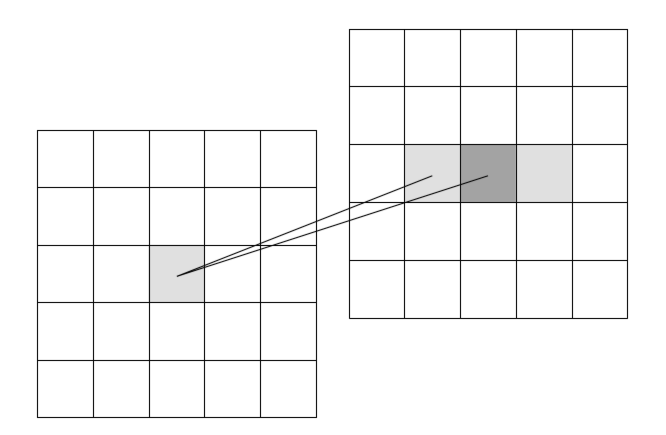
\includegraphics[width = \textwidth]{Pictures/deformation/cluster_1x1.png}
         \caption{One pixel per cluster.}
      \end{subfigure}
      \quad
       %add desired spacing between images, e. g. ~, \quad, \qquad, \hfill etc. 
        %(or a blank line to force the subfigure onto a new line)
      \begin{subfigure}[t]{0.45\textwidth}
        \centering
        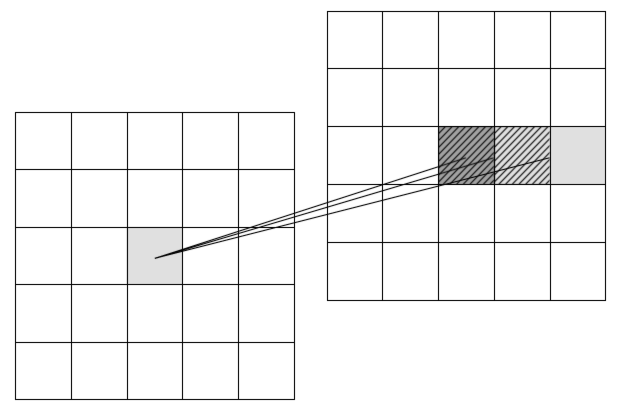
\includegraphics[width = \textwidth]{Pictures/deformation/cluster_1x2.png}
        \caption{$1 \times 2$ pixels per cluster.}
      \end{subfigure}
      
      \begin{subfigure}[t]{0.45\textwidth}
        \centering
        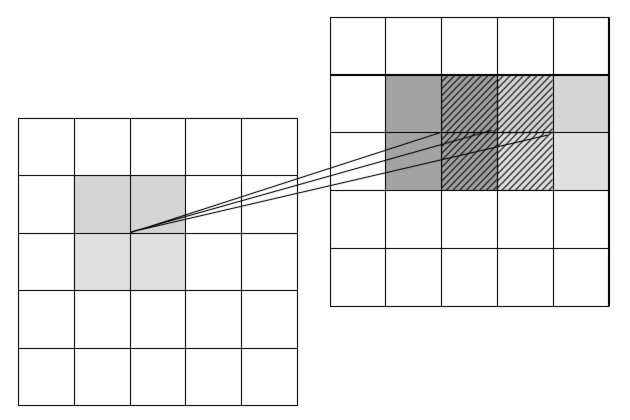
\includegraphics[width = \textwidth]{Pictures/deformation/cluster_2x2.png}
        \caption{$2 \times 2$ pixels per cluster.}
      \end{subfigure}
      \quad
      \begin{subfigure}[t]{0.45\textwidth}
        \centering
        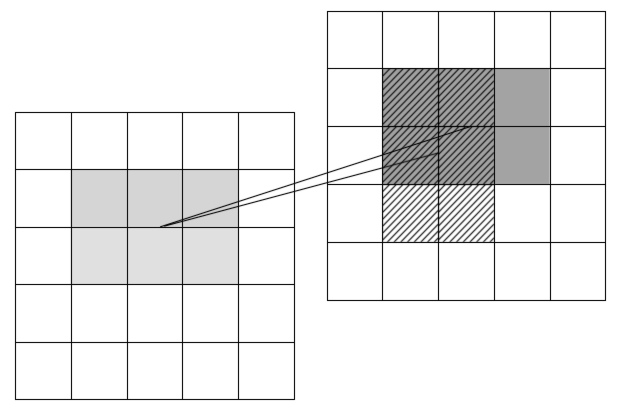
\includegraphics[width = \textwidth]{Pictures/deformation/cluster_3x3.png}
        \caption{$3 \times 3$ pixels per cluster.}
      \end{subfigure}
      \caption{Minimum distance between the cluster projected on one side to the position of the cluster of this side.}
      \label{fig:clusterSize}
   \end{figure}

   Hence, for one pixel clusters, the displacement between the two pixels is the pitch $p = 18.4 \text{ }\mu\text{m}$ and the angle between the two minimal hit position is then $\theta \sim 0.52^{\degree}$.
   A selection of the events where only clusters of 1 pixel are considered is shown on the figure~\ref{fig:angRes1x1}.
   The two peaks have a spacing closed to $0.5^{\degree}$.


   \begin{figure}[!h]
     \centering
      \begin{subfigure}[t]{0.45\textwidth}
         \centering
         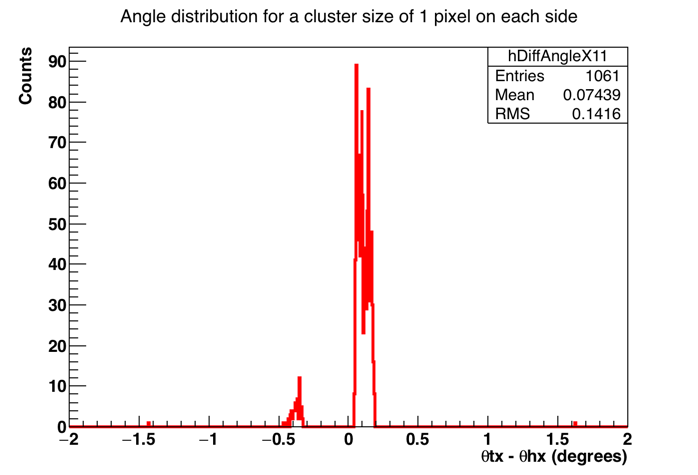
\includegraphics[width = \textwidth]{Pictures/deformation/hDiffAngleX11_226056.png}
         \caption{One pixel per cluster.}
         \label{fig:angRes1x1}
      \end{subfigure}
      \quad
       %add desired spacing between images, e. g. ~, \quad, \qquad, \hfill etc. 
        %(or a blank line to force the subfigure onto a new line)
      \begin{subfigure}[t]{0.45\textwidth}
        \centering
        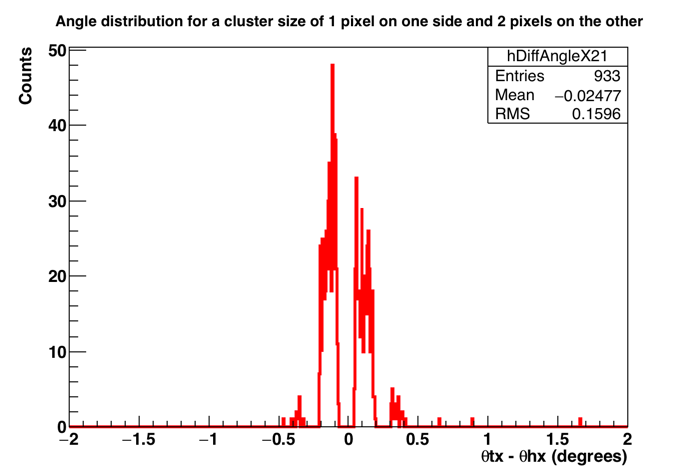
\includegraphics[width = \textwidth]{Pictures/deformation/hDiffAngleX21_226056.png}
        \caption{$2 \times 1$ pixels per cluster.}
        \label{fig:angRes2x2}
      \end{subfigure}
      
      \begin{subfigure}[t]{0.45\textwidth}
        \centering
        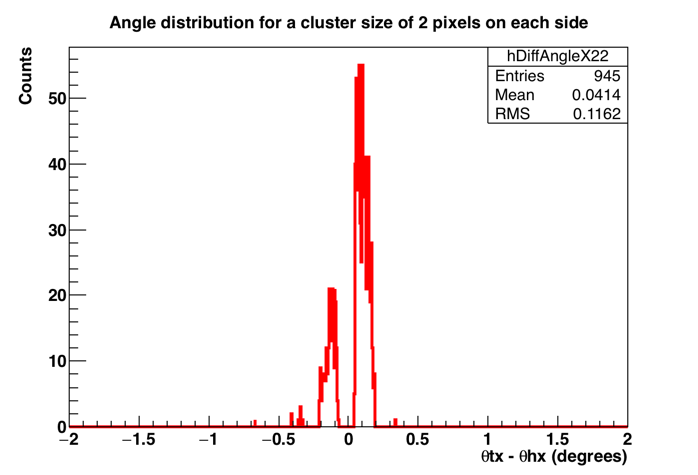
\includegraphics[width = \textwidth]{Pictures/deformation/hDiffAngleX22_226056.png}
        \caption{$2 \times 3$ pixels per cluster.}
        \label{fig:angRes2x3}
      \end{subfigure}
      \quad
      \begin{subfigure}[t]{0.45\textwidth}
        \centering
        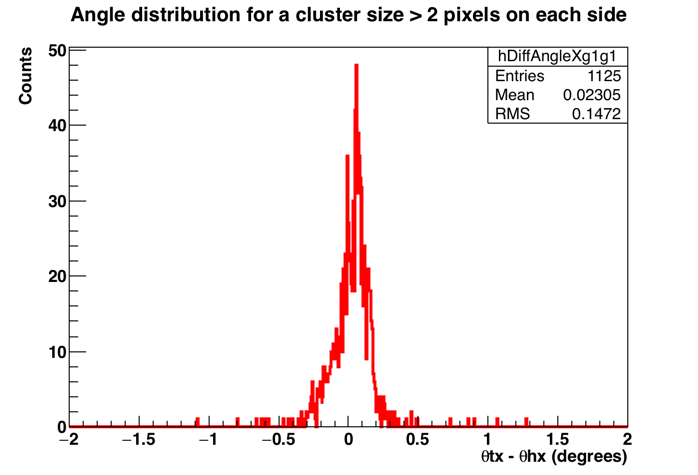
\includegraphics[width = \textwidth]{Pictures/deformation/hDiffAngleXg1g1_226056.png}
        \caption{Clusters bigger than $2 \times 2$ pixels.}
      \end{subfigure}
      \caption{Minimum distance between the cluster projected on one side to the position of the cluster of this side.}
      \label{fig:anglResDecomposed}
   \end{figure}
   

